% datum{16. Oktober 2015}

\section{Einleitung}
\label{sec:einleitung}

\subsection{Beispiele}
\label{sec:beispiele}

\begin{enumerate}
\item Navier Stokes Gleichungen

  \begin{align*}
    \underbar u =
    \begin{pmatrix}
      u_{1}(x, t)\\
      u_{2}(x, t)
    \end{pmatrix} \qquad &\text{Geschwindigkeit}\\
p = p(x, t) \qquad &\text{Druck}, 
  \end{align*}
  \begin{subequations}
\label{eq:ns}
  \begin{align}
    u_{t} + (u\cdot \nabla)u - \frac 1 R \Delta u + \nabla p = 0\quad &\text{in } \Omega_{T} = \Omega \times [0, T] \label{eq:ns1}\\
\nabla\cdot u = 0 \quad &\text{in } \Omega_{T} \label{eq:ns2}
  \end{align}
  \end{subequations}
  \begin{subequations}
    \label{eq:ns}
    \begin{align}
      u|_{\partial \Omega} = u_{d} \quad &\text{in } [0, T]\label{eq:ns_rb}\\
      u(\cdot, 0)= u_{0} \quad &\text{in } \Omega \label{eq:ns_ab}
    \end{align}
  \end{subequations}

mit der Reynoldszahl $R >> 1$ (bei uns, das entspricht einer turbulenten Strömung). 

Es sind $u\cdot \nabla = u_{1}\partial_{x} + u_{2} \partial_{y}$ und $\Delta = \partial_{x}^{2} + \partial_{y}^{2} $ Operatoren. 

Zu \eqref{eq:ns1} Momentenerhaltung:
\begin{align*}
  \partial_{t}u_{1} + u_{1}\partial_{x}u_{1} + u_{2}\partial_{y}u_{1} -\frac 1 R \Delta u_{1} + \partial_{x} p = 0\\ 
  \partial_{t}u_{2} + u_{1}\partial_{x}u_{2} + u_{2}\partial_{y}u_{2} -\frac 1 R \Delta u_{2} + \partial_{y} p = 0
\end{align*}
stammt von $\partial_{t} u + \underbrace{\nabla\cdot(uu)}_{\text{Moment}} + \underbrace{\nabla p}_{\text{Druckänderung}}-\frac 1 R  \underbrace{\Delta u}_{\text{Diffusion}}  = 0$

Zu \eqref{eq:ns2} Masse-/Volumenerhaltung
\begin{align*}
  \partial_{x} u_{1} +   \partial_{y} u_{2} = 0 \iff \text{ Annahme: Inkompressibilität und konstante Dichte}
\end{align*}
Die Navier-Stokes-Gleichungen sind ein nichtlineares System von zeitabhängigen, partiellen Differentialgleichungen. 

Linearisierung von $(u\cdot\nabla)u$ zu $(b\cdot\nabla)u$ und weitere Vereinfachungen ($u_{1} = u_{2}$, $p = 0$) führen zu 
\begin{align*}
    u_{t} + \underbrace{\eps\Delta u}_{\text{Diffusion}} + \underbrace{(b\cdot\nabla)u}_{\text{Konvektion}} + \underbrace{cu}_{\text{Reaktion}} = f&\quad \text{in } \Omega_{T}\\
u|_{\partial \Omega} = 0& \quad \text{in } [0, T]\\
u(\cdot, 0) = u_{0}&
\end{align*}
mit $0 < \eps = \frac 1 R \ll 1$. 
Ein solches $\eps$ kommt immer bei singulär gestörten Problemen vor. Wenn $\eps$ gegen $1$ geht, ist es eine Differentialgleichung zweiter Ordnung, wenn $\eps$ gegen $0$ geht, ist es eine Differentialgleichung erster Ordnung. Diese haben verschiedene Anforderungen an die Rand- und Anfangsbedinungen!

Die Problemklasse heißt \markdef{Konvektions-Diffusions-Probleme} und $\eps$ ist der (singuläre) \markdef{Störungsparameter}. Das zugehörige stationäre Problem ($u_{t} = 0$) ist
\begin{align*}
   -\underbrace{\eps\Delta u}_{\text{Diffusion}} + \underbrace{b\cdot\nabla u}_{\text{Konvektion}} + \underbrace{cu}_{\text{Reaktion}} = f&\quad \text{in } \Omega\\
u|_{\partial \Omega} = 0& 
\end{align*}
Wenn $\nnorm b \gg \eps > 0$, so  dominiert die Konvergenz, wenn $\nnorm b = 0$, $c > 0$ so dominiert die Reaktion. 
\item Modellierung eines Strömungsreaktors ($\sim$ 1D)

Gegeben: Ein Rohr der Länge $L$, in das die Reaktionsmasse eingeht und die Produkte rauskommen. 
Stoffbilanz:
\begin{align*}
  c_{t} = - \nabla \cdot(v c) + D \nabla c + r(c) \In \Omega_{T} = \Omega \times [0, T]
\end{align*}
mit
\begin{itemize}
\item $c = c(x, t)$ Konzentration, 
\item $v = (v_{1}(x, t), \dots, v_{d})^{T}(x, t))$ Geschwindigkeitsfeld, 
\item $r(c)$ Reaktionsterm, 
\item $D$ Diffusionskoeffizient. 
\end{itemize}
Eindimensionales Modell ($L \ll 1$, $v$ zeitlich konstant):
\begin{align*}
  c = c(x) \, (\to c_{t} = 0), &\\
0 = - Dc'' + vc' + r(c)& \In (0, L). 
\end{align*}
Einführung dimensionsloser Größen:
\begin{align*}
  J &= \frac x L, \quad u = \frac c c_{0} \in [0, \infty) \\
\implies \quad \frac{c(x)}{c_{0}} &= \frac{J\cdot L}{c_{0}} = u(J)\\
\implies \quad \frac{dc}{dx} &= \frac{du }{d\xi} \frac{d\xi}{dx}\cdot c_{0} = u'(\xi) \frac{c_{0}}{L}\\
\frac{d^{2}c}{dx^{2}} &= u''(\xi) \frac{c_{0}}{L^{2}}\\
\implies \quad 0 &= - \frac{Dc_{0}}{L^{2}} + \frac{V c_{0}}{L} u' + \underbrace{r (u c_{0})}_{R(u)}\\
\iff \quad 0 &= - \frac{D}{V\cdot L}u'' + u' + R(u). 
\end{align*}
Die Peclét-Zahl $Pe= \frac{V\cdot L} D$ misst das Verhältnis zwischen Konvektion und Diffusion. Mit $\epsilon = \frac 1 {Pe}$ und $L \ll1$ folgt $0< \epsilon \gg1$ und
\begin{align*}
  - \epsilon u'' + u' + R(u) = 0 & \In (0, 1)\\
+ \text{Randbedingungen} &
\end{align*}
\item Mathematisches Beispiel
  \begin{subequations}
\label{eq:3}
  \begin{align*}
    - \epsilon u'' + u' = 1 & \In (0, 1)\\
u(0) = u(1) = 0. 
  \end{align*}
  \end{subequations}
Sei (wie meistens) $0< \epsilon \ll 1$. Dann ist \eqref{eq:3} eine lineare Differentialgleichung zweiter Ordnung, inhomogen, ein Randwertproblem und hat konstante Koeffizienten. Lösungsansatz über die charakteristische Lösung:
\begin{itemize}
\item Homogene Gleichung:
  \begin{align*}
    u &= e^{\lambda x}\\
    - \epsilon \lambda^{2} - \lambda &= 0\\
u_{hom} &= c_{1} + c_{2} \cdot e^{- \frac 1 \epsilon x}.  
  \end{align*}
\item Variation der Konstanten:
  \begin{align*}
    u_{p} = A\cdot x = - x
  \end{align*}
\item Allgemeine Lösung:
  \begin{align*}
    u = c_{1} + c_{2} \cdot e^{- \frac x \epsilon} - x. 
  \end{align*}
\item Randbedingungen nutzen:
  \begin{align*}
    u(x) = \frac{1 - e^{- \frac x \epsilon}}{1 - e^{- \frac 1 \epsilon}} - x
  \end{align*}
löst \eqref{eq:3}. 

Skizzen 1 , 2, 3
\end{itemize}
Nun wählen wir 
\begin{itemize}
\item $x_{0} \in (0, 1]$:
\begin{align*}\left. 
  \begin{aligned}
    \lim_{x \to x_{0}} \lim_{\epsilon \to 0} u(x) &= \lim_{x \to x_{0}} (1 - x) = 1 - x_{0}\\
    \lim_{\epsilon \to 0} \lim_{x \to x_{0}} u(x) &= \lim_{ \epsilon \to 0} \(\frac {1 - e^{- \frac {x_{0}} \epsilon}}{1 - e^{- \frac 1\epsilon}} - x_{0}\) = 1 - x_{0}
  \end{aligned} \right\}\text{Grenzschichten dürfen vertauscht werden}
\end{align*}

\item $x_{0} = 0$:
\begin{align*}\left. 
  \begin{aligned}
    \lim_{x \to x_{0}} \lim_{\epsilon \to 0} u(x) &= \lim_{x \to 0} (1 - x) = 1\\
    \lim_{\epsilon \to 0} \lim_{x \to x_{0}} u(x) &= \lim_{ \epsilon \to 0}  0 = 0
  \end{aligned} \right\}\text{Grenzprozesse dürfen nicht vertauscht werden}. 
\end{align*}
\end{itemize}
\item Zentrales Differenzenverfahren mit $u_{i} \approx u(x_{i}), \quad x_{i} = i\cdot h, \quad h = \frac 1 N$
  \begin{align*}
    - \frac \epsilon {h^{2}} (u_{i-1} - 2u_{i} + u_{i+1})- \frac {u_{i+1} - u_{i-1}} {2\cdot h} &= 1, \quad i = 1, \dots, N-1,\\
u_{0} = u_{N} &= 0. 
  \end{align*}
Differenzengleichung ist 'diskretisiert', linear, zweiter Ordnung und homogen. Ansatz für homogenes Problem: $u_{i} = \lambda^{i}$, löse partikuläres Problem nach rechter Seite $u_{i} = a \cdot i$. Lösungen:
\begin{align*}
  \lambda_{1} &= 1\\
   \lambda_{2} &= \frac{2 \epsilon - h}{2 \epsilon + h} \eqqcolon \lambda\\
   u_{i} &= \frac{1 - \lambda^{i}}{1 - \lambda^{N}} - i\cdot h, 
\end{align*}
aber $\lambda < 0$ fpr $h > 2 \epsilon$, was meistens erfüllt ist. Also oszilliert $\lambda^{i}$ und die diskrete Lösung, aber die stetige Lösung ist glatt. 

\begin{figure}[h!]
  \centering
  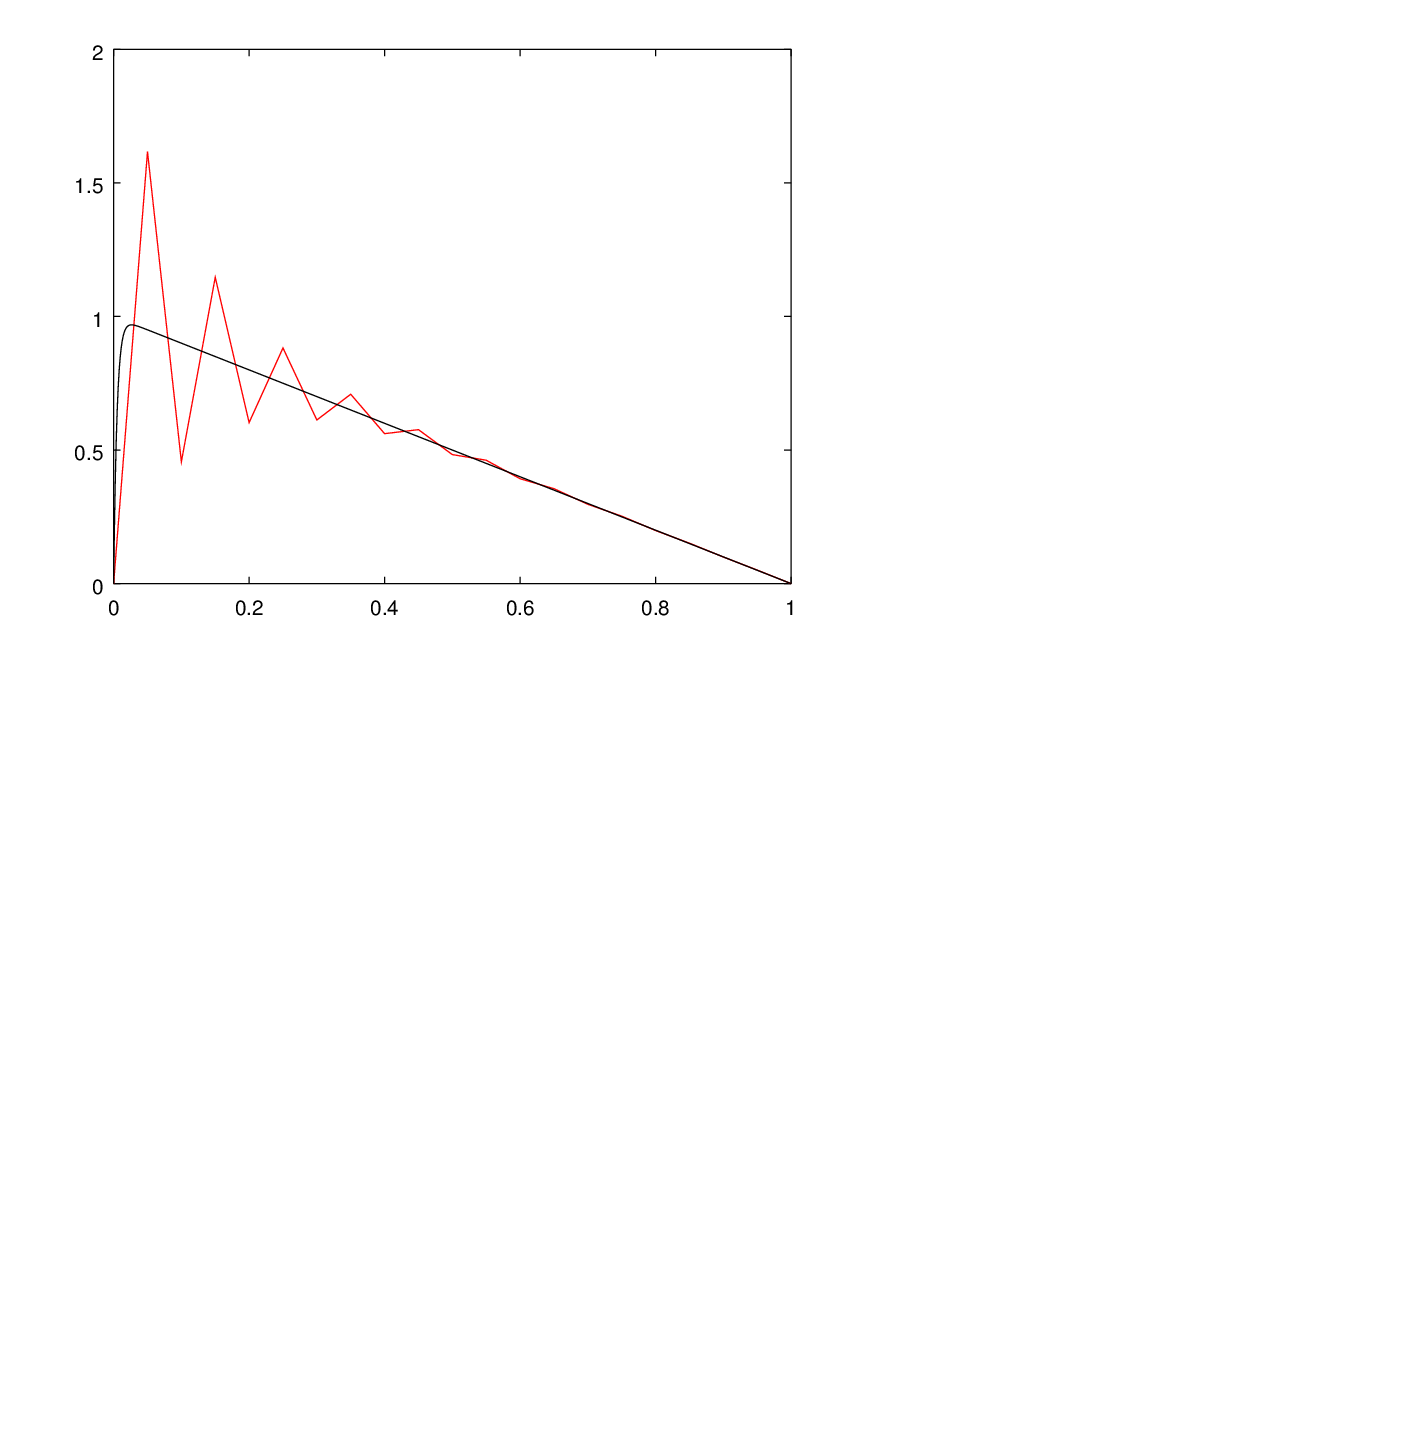
\includegraphics[scale=0.4]{1_oscillating.png}
%  \begin{tikzpicture}
%    \draw ‎[‎smooth,‎samples=100‎,domain=0:‎‎1‎‎] ‎plot
%    \draw[‎smooth,‎samples=100‎,domain=0:‎‎1‎‎] ‎plot({\x},‎‎‎‎‎‎‎‎{\x});
%     \def\eps {0.005};
%     \def\n{30};
%     \def\l{(2*\eps - 1/\n)/(2*\eps + 1/\n)};
%     \def\e{2.71828};

%     \draw[->] (0,0) -- (2,0) node[right] {$x$};
%     \draw[->] (0,0) -- (0,2) node[above] {$y$};
%     \draw[domain=0:1, samples= \n, variable=\x, blue] plot ({\x}, {1 - \l^(\x)/(1 - \l^(\n))});

%     \draw[domain=0:1, smooth, variable=\x, red] plot ({\x}, {(1 - e^(- \x/\eps))/(1 - e^(- 1/\eps)) - \x}) ;
%     \def\eps{0.2};
%     \draw[domain=0:1, smooth, variable=\x, red] plot ({\x}, {(1 - e^(- \x/\eps))/(1 - e^(- 1/\eps)) - \x}) ;
%     \def\eps{0.4};
%     \draw[domain=0:1, smooth, variable=\x, red] plot ({\x}, {(1 - e^(- \x/\eps))/(1 - e^(- 1/\eps)) - \x}) ;

% %    \draw[domain=0:1, smooth, variable=\x] plot ({\x}, {1 - \l^(\n)});
%   \end{tikzpicture}
  \caption{Veranschaulichung der diskreten und stetigen Lösung}
  \label{fig:oscillations}
\end{figure}

Betrachte $x_{1} = h$ für $h = \epsilon$, $u_{1} = \frac {1 - \lambda}{1 - \lambda^{N}} - h$, $\lambda = \frac 13$. Dann
\begin{align}
  u_{1} = \frac {\frac 23}{1 - \lambda^{N}} - \frac 1N \to \frac 23 \quad (N \to \infty, \, h \to 0,\,  \epsilon \to 0). 
\end{align}
Exakt:
\begin{align*}
  u(x_{1}) = \frac {1 - e^{ - \frac h \epsilon}}{1 - e^{- \frac 1 \epsilon}} - \frac 1 N \to 1 - \frac 1 e \quad (N \to \infty, \, h \to 0,\,  \epsilon \to 0). 
\end{align*}


\end{enumerate}

\subsection{Definitionen singulär gestörter Probleme}
\begin{definition}
  Ein Problem heißt \markdef{singulär gestört}, falls ein $\hat x \in \bar \Omega$ existiert, sodass
  \begin{align*}
    \lim_{\epsilon \to 0} \lim_{x \to \hat x} u(x) \neq \lim_{x \to \hat x} \lim_{\epsilon \to 0}  u(x) 
  \end{align*}
gilt. Etwas formaler sei
\begin{align}\label{eq:4}
  \cL u_{\epsilon} &= h(x, \epsilon) \in \Omega \quad \text{in } \Omega\\
  \cB u_{\epsilon} &= 0 \quad \text{auf } \partial \Omega \notag
\end{align}


\begin{align*}
  \cL u_{\epsilon} = h(x, \epsilon) \in \Omega \quad &\text{in } \Omega\\
  \cB u_{\epsilon} = 0 \quad &\text{auf } \partial \Omega 
\end{align*}


eine (partielle) Differentialgleichung mit Randbedingung,  $\nnorm {\cdot}$ eine Norm mit $\lim_{\epsilon \to 0} \nnorm{u_{\epsilon}} \neq 0$, eine Aufspaltung $\cL = \cL_{0} + \epsilon \cL_{p}$ mit $\cL_{0}$ und $\cL_{p}$ unabhängig von $\epsilon$, $\cL_{0}$ erfüllt (einen Teil) der Randbedingungen. 
\end{definition}
\begin{definition} \label{def:1-2}
  Das Problem \eqref{eq:4} heißt \markdef{regulär gestört}, falls es eine Funktion $\phi_{0}$ unabhängig von $\epsilon$ gibt, sodass $\cL_{0}\phi_{0} = h(x, 0)$ und $\lim_{\epsilon\to 0} \nnorm{u_{\epsilon} - \phi_{0}} = 0$ gilt. 

Ansonsten heißt \eqref{eq:4} \markdef{regulär gestört}. 
\end{definition}
Es können nicht nur Differentialgleichungen gestört sein, sonder auch algebraische Gleichungen etc.

\begin{bemerkung}
  Die Definition \ref{def:1-2} ist normabhängig. \eqref{eq:3} ist regulär gestört in $\nnorm \cdot_{L_{1}}$, da
  \begin{align*}
    \nnorm{u_{\epsilon}}_{L_{1}} = \int_{0}^{1}\( \frac{1 - e^{- \frac x \epsilon}}{1 - e^{- \frac 1 \epsilon}} - x \) = \frac {1 + \epsilon \(e^{- \frac 1 \epsilon} -1 \)}{1 - e^{- \frac 1 \epsilon}} - \frac 12 \to \frac 12 \neq 0 \quad(\epsilon \to 0). 
  \end{align*}
Aus $-u' = 1$ und $u(1) = 0$ folgt $\phi_{0} = 1- x$. 
\begin{align*}
      \nnorm{u_{\epsilon}-\phi_{0}}_{L_{1}} = \int_{0}^{1}\( \frac{1 - e^{- \frac x \epsilon}}{1 - e^{- \frac 1 \epsilon}} - 1 \) = \frac {e^{-\frac{1}{\epsilon}} + \epsilon \(e^{- \frac 1 \epsilon} -1 \)}{1 - e^{- \frac 1 \epsilon}}  \to \frac 12 \neq 0 \quad(\epsilon \to 0). 
\end{align*}

\eqref{eq:3} ist singulär gestört bezüglich $\nnorm \cdot_{L_{\infty}}$, da $\nnorm {u_{\epsilon}}_{L_{\infty}} > 0$ ($u_{\epsilon}$ ist immer positiv in $(0, 1)$) und
\begin{align*}
      \nnorm{u_{\epsilon}}_{L_{\infty}} = \nnorm{ \frac{e^{- \frac 1 \epsilon} - e^{- \frac x \epsilon}}{1 - e^{- \frac 1 \epsilon}}}_{L_{\infty}} \geq \norm{ \frac{e^{- \frac 1 \epsilon} - e^{- \frac 0 \epsilon}}{1 - e^{- \frac 1 \epsilon}}}_{L_{\infty}} = 1. 
\end{align*}
\eqref{eq:3} ist regulär gestört bezüglich $\nnorm \cdot_{L_{2}}$, aber singulär gestört bezüglich $\norm \cdot_{H^{1}} = \nnorm{\nabla\cdot}_{L_{2}}$. 
\end{bemerkung}

Der uns interessierende Fall wird sein, dass $\cL_{p}$ ein Differentialoperator höherer Ordnung und $\cL_{0}$ ein Differentialoperator niedrigerer Ordnung ist. 

%%% Local Variables: 
%%% mode: latex
%%% TeX-master: "vorlesung"
%%% End: 
